\chapter{analysis}\label{analysis}

ToDo:
\begin{enumerate}[nosep]
    \item Datenformat Input, verwendete Daten, Worte zu Simulation, trainingsdaten
    \item Preprocessing - Schritte erklären
    \item Datenformat Output Preprocessing
    \item ...
    \item Anwendung Random Forests mono, disp erklären anhand hillas parameter
    \item Anwendung Stereo (Random forest, stabile Mittelwertverfahren -alle erklären)
    \item Signifikanzkurve
\end{enumerate}

\section{Data Levels, preprocessing}

\subsection{DL0, simtel}
At the lowest level our observed data consists of uncalibrated waveforms 
in the camera pixels.

\subsection{From Dl0 to DL1}

- calibration
- cleaning
- hillas parameters 
- telescope level



\begin{figure}
    \begin{subfigure}{0.3\textwidth}
        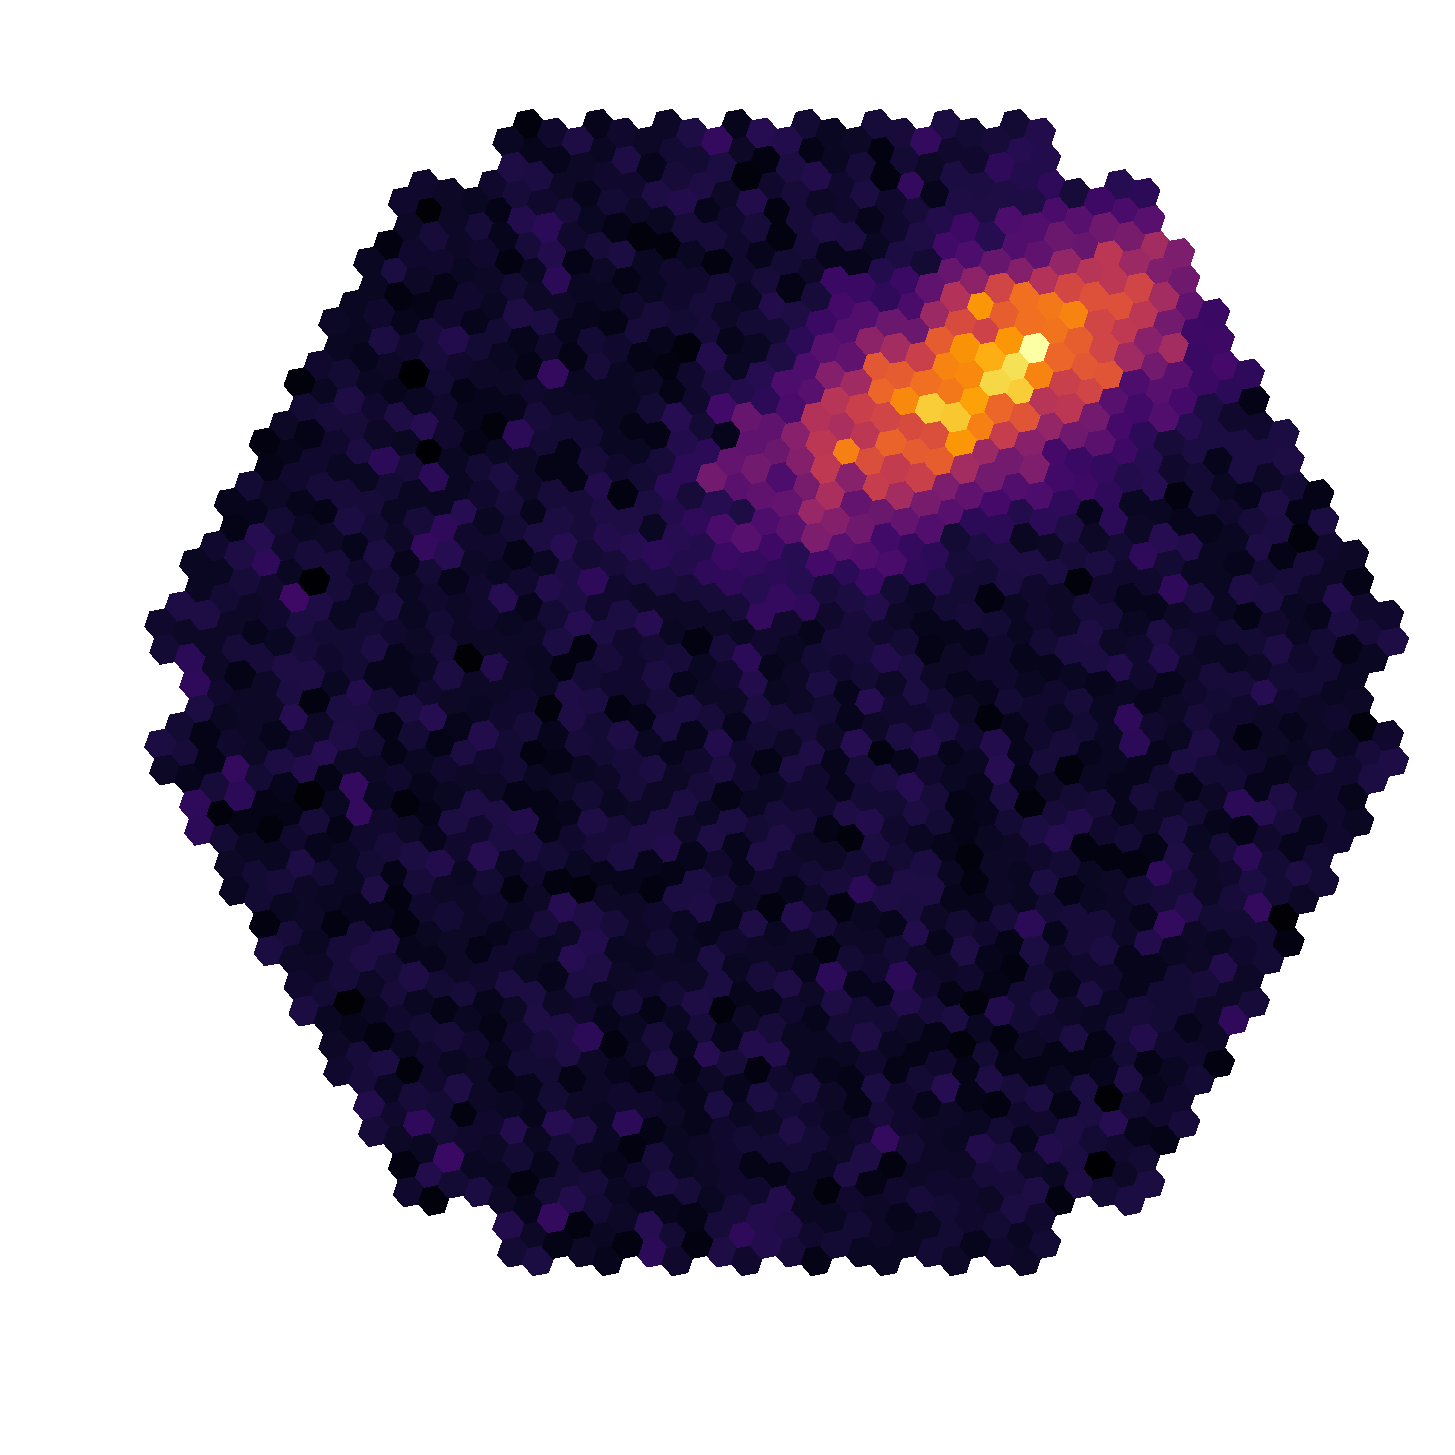
\includegraphics[width=0.9\linewidth]{../Plots/hillas_raw.pdf} 
        %\caption{Caption1}
        \label{fig:shower_image_raw}
    \end{subfigure}
    \begin{subfigure}{0.3\textwidth}
        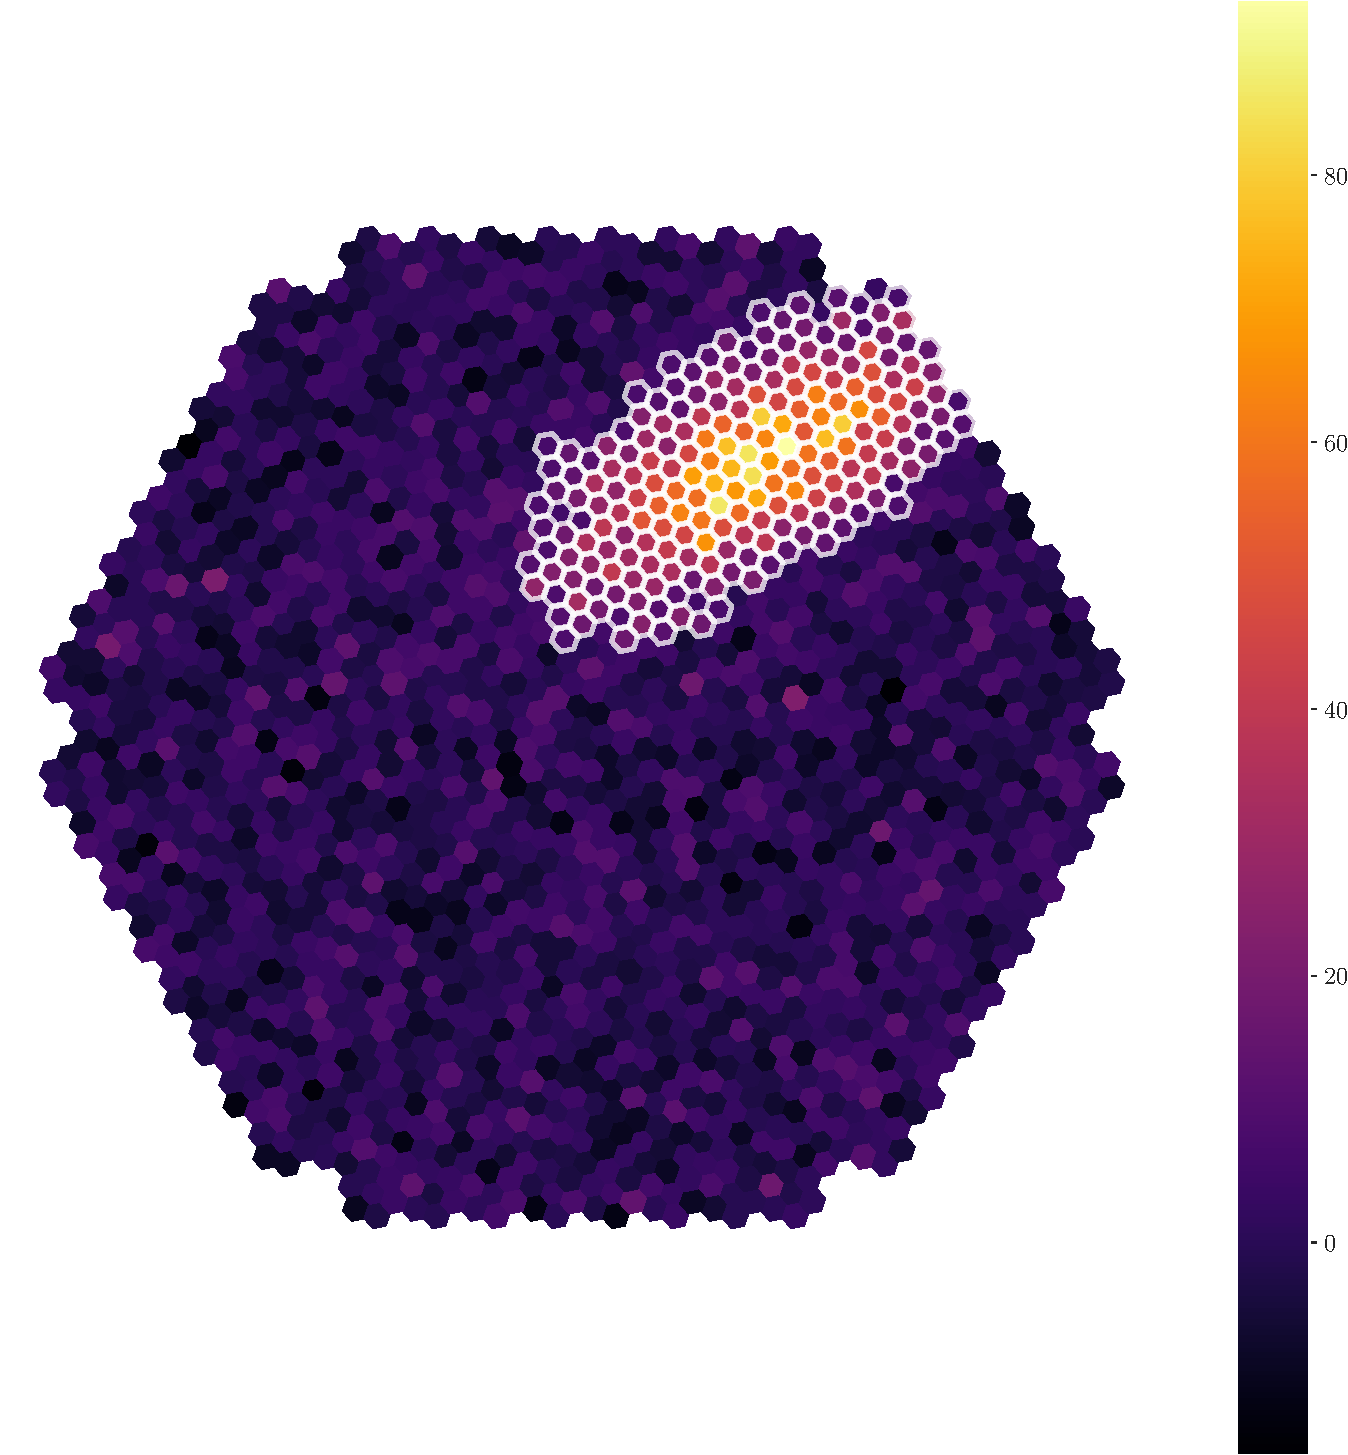
\includegraphics[width=0.9\linewidth]{../Plots/hillas_cleaned.pdf}
        %\caption{Caption 2}
        \label{fig:shower_image_cleaned}
    \end{subfigure}
    \begin{subfigure}{0.3\textwidth}
        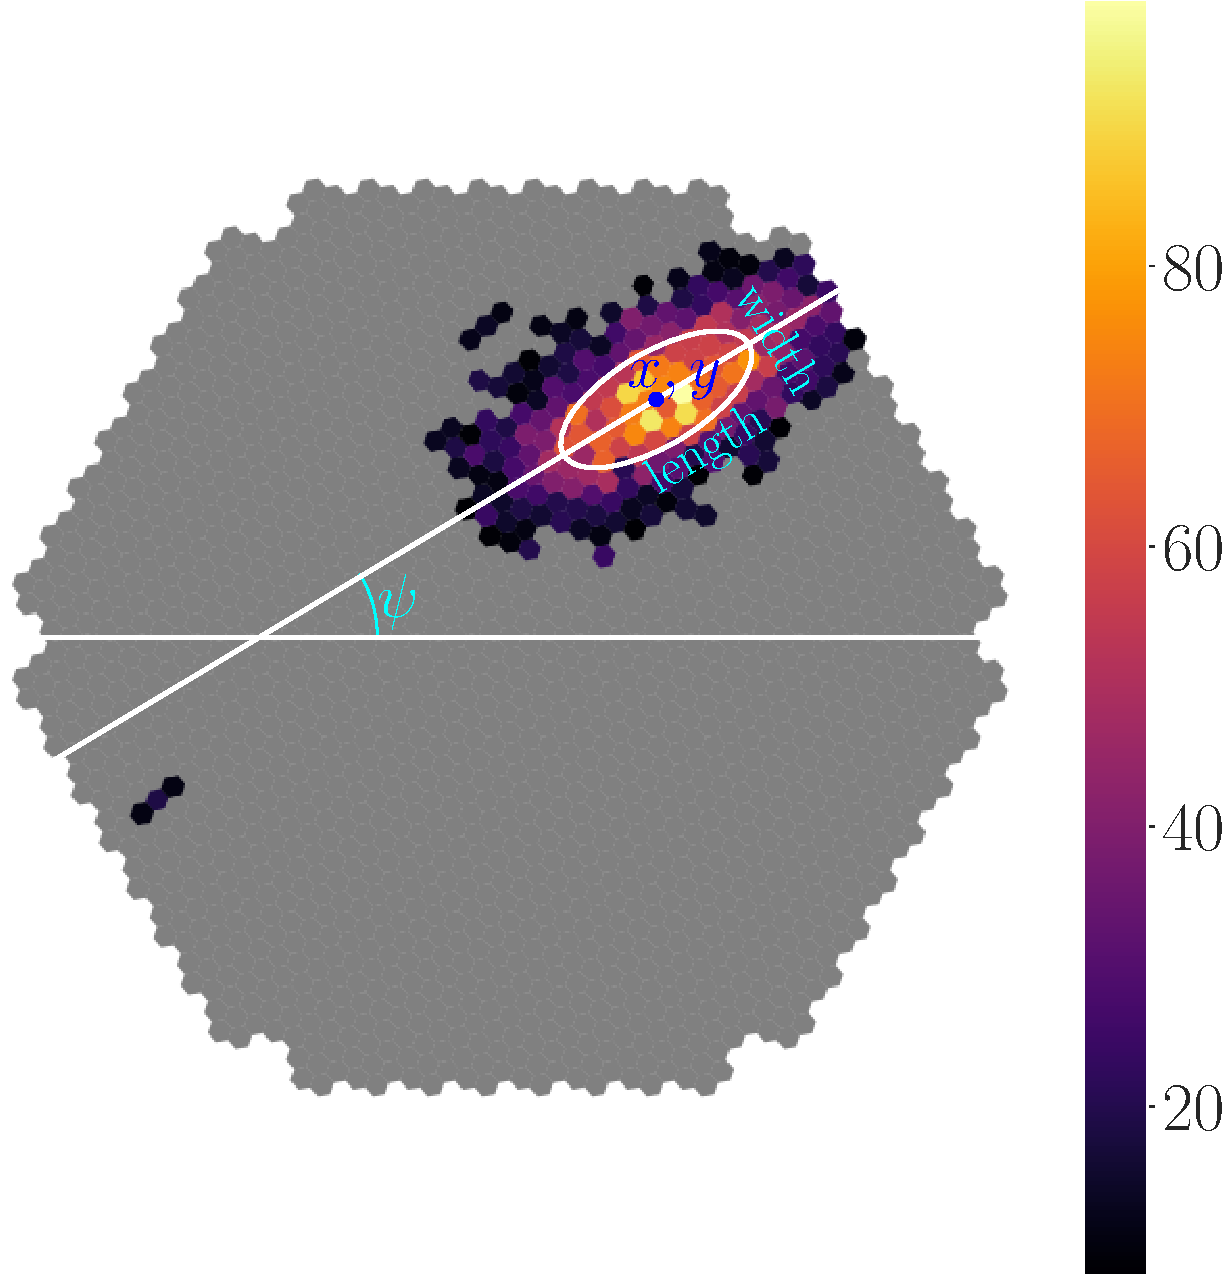
\includegraphics[width=0.9\linewidth]{../Plots/hillas_cleaned_params.pdf} 
        %\caption{Caption1}
        \label{fig:hillas_parameters_only}
    \end{subfigure}
    \caption{Illustration of a simulated gamma shower captured with the LST-telescope.
        The left figure shows the image after applied waveform-extraction but before
        the cleaning step. The right figure shows the image after the cleaning has been applied
        and non-selected pixels have been discarded.}
    \label{fig:shower_image}
\end{figure}

\subsection{From DL1 to DL2}  % we dont seperate between 0 and 1 right?
erklären, dass hillas reco reinkommt -> stereo features

\subsection{Machine Learning, dl3?}
High level analysis of the preprocessed data is based on the use of
the aict-tools \cite{aict-tools} package which is based on
sklearn \cite{sklearn_api} for the machine learning algorithms.
The algorithm of choice is the Random Forest algorithm
as it is well suited for the use with tabluar data and tends to not overfit
(citation needed).
Seperate models are trained for the tasks of signal/background
separation, signal energy estimation and signal source position
reconstruction.
The aict-tools have originally been developed for the FACT-experiment
(citation needed) which is a single IACT. For this reason
different ways of combining the results from single telescopes events
to stereo events will be presented.


\section{g/h sep}
For the task of gamma/hadron separation a random forest can be trained
using either only monoscopic information or also using array-level
information from earlier reconstruction steps.
This generally improves the accuracy by a few percent.
The single telescope predictions can be combined by
simple functions such as the mean or median of the
single predictions to provide a prediction for the complete
array-event.
Alternatively the single telecope predictions can be used to
feed a second random forest to provide array-level predictions.
Such a second model can easily be trained on array-level
features, e.g. mean and std of the single predictions, number of triggered
telescopes, total luminosity or features calculated from the
Hillas-Reconstructor if not already used for the single telescope
prediction. in this case the model would effectively deviate
from the mean of the prediction according to information that the
single predictions did not include.


STEREO IN REKONSTRUKTION EINBAUEN??


\section{energy estimation}
Energy estimation can be performed in the same way as the gamma/hadron
separation. For this task there has been earlier work indicating
the usefulness of a second machine learning model trained
on the predictions of the first telesope-level model
\cite{ba-lars}.

I am thus going to present results based on either calculating the mean
of the telescope level predictions and using a second random forest
to improve the array level prediction.

\section{source position}
\label{sec:source_position}
Given the source position in the camera frame the source position
on the sky can be calculated with coordinate transformations if
the position, pointing and optical properties of the
telescope are known.
In general the true source position in the camera frame is assumed to be
different from the center of gravity of the shower ellipse
but located somewhere along the main shower axis.
The position on the shower axis can be estimated based on 
the hillas parameters and other image features.
This method is known as the DISP-method in the
literature (citation needed). The general idea 
can be seen in figure \ref{fig:disp}.

\begin{figure}
    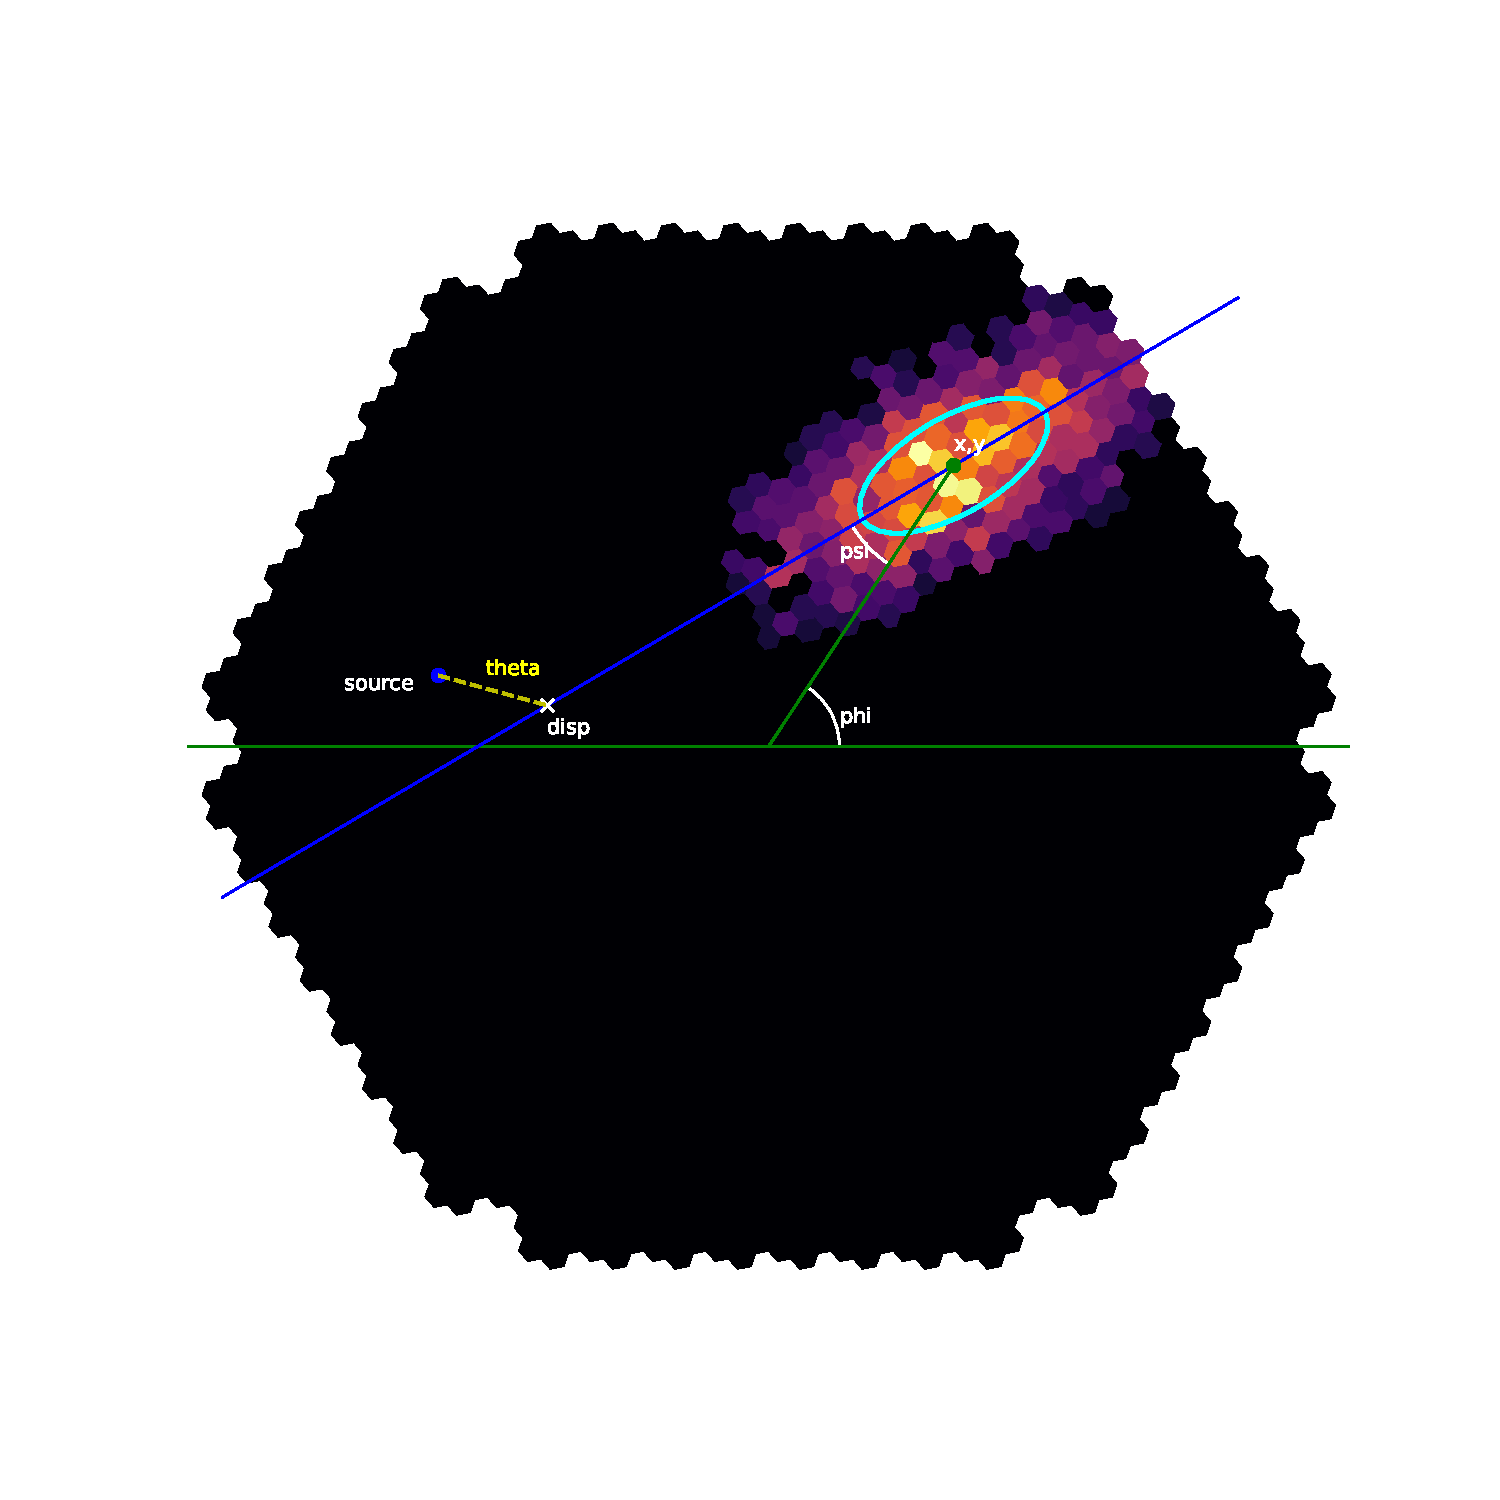
\includegraphics[width=0.9\linewidth]{../Plots/hillas_complete.pdf}
    \caption{Illustration of monoscopic source position reconstruction making use of 
        the Hillas-Parameters and the DISP-method as explained in section \ref{sec:source_position}.
        The left figure has the hillas ellipse and parameters drawn onto our previously cleaned sample shower.
        The right figure estimates a source Position in the Camera frame.}
    \label{fig:disp}
\end{figure}

With the DISP-method the estimated distance between the source
position and the center of gravity of the hillas ellipse gets calculated
based on the form of the ellipse, timing information and potentially
more features.
This can be done analitically, via lookup-tables or with machine learning.
At this point the reconstructed source position
is fixed at two points at the main shower axis, see figure \ref{fig:disp_amb}


\begin{figure}
    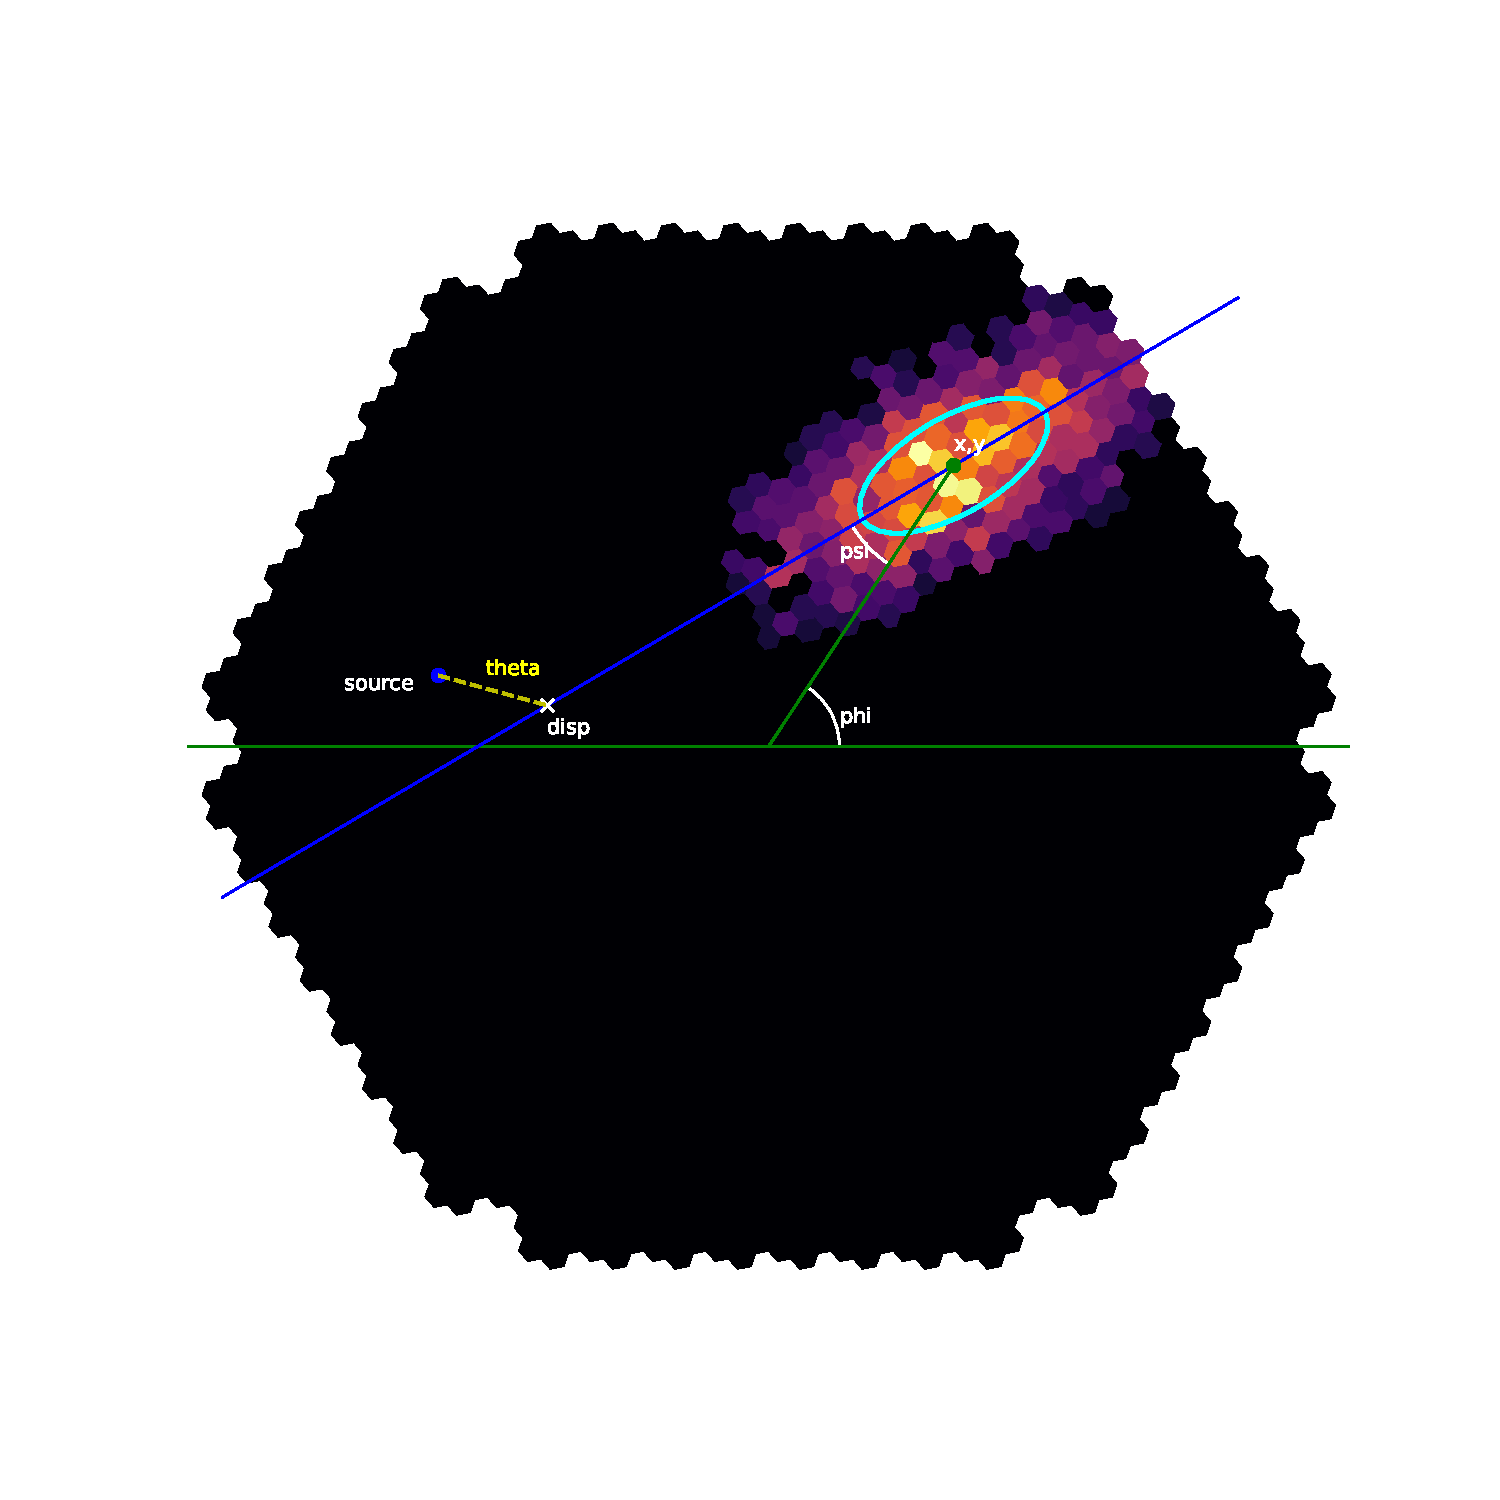
\includegraphics[width=0.9\linewidth]{../Plots/hillas_complete.pdf}
    \caption{Wrong pic!}
    \label{fig:disp_amb}
\end{figure}


The remaining task then consists of finding the correct one of these
two points. If there is no stereoscopic information available,
a choice can be made based on the image features again.
In FACT-analyses a second random forest is trained for this
specific purpose, usually yielding an accuracy around 70-80\% (citation).
This is called SIGN-prediction, interpreting the two possible sides
as +-1.
In the case of the MAGIC-telescopes the ambiguity does not
get resolved until the individual results get combined
to the stereo level. The choice of the correct
pair out of the four reconstructed positions can be done either
by calculating the crossing point of both main shower axises
or by calculating the pairwise distances between the positions (citation).


These methods are illustrated in figure \ref{fig:disp_magic}


\begin{figure}
    \begin{subfigure}{0.3\textwidth}
        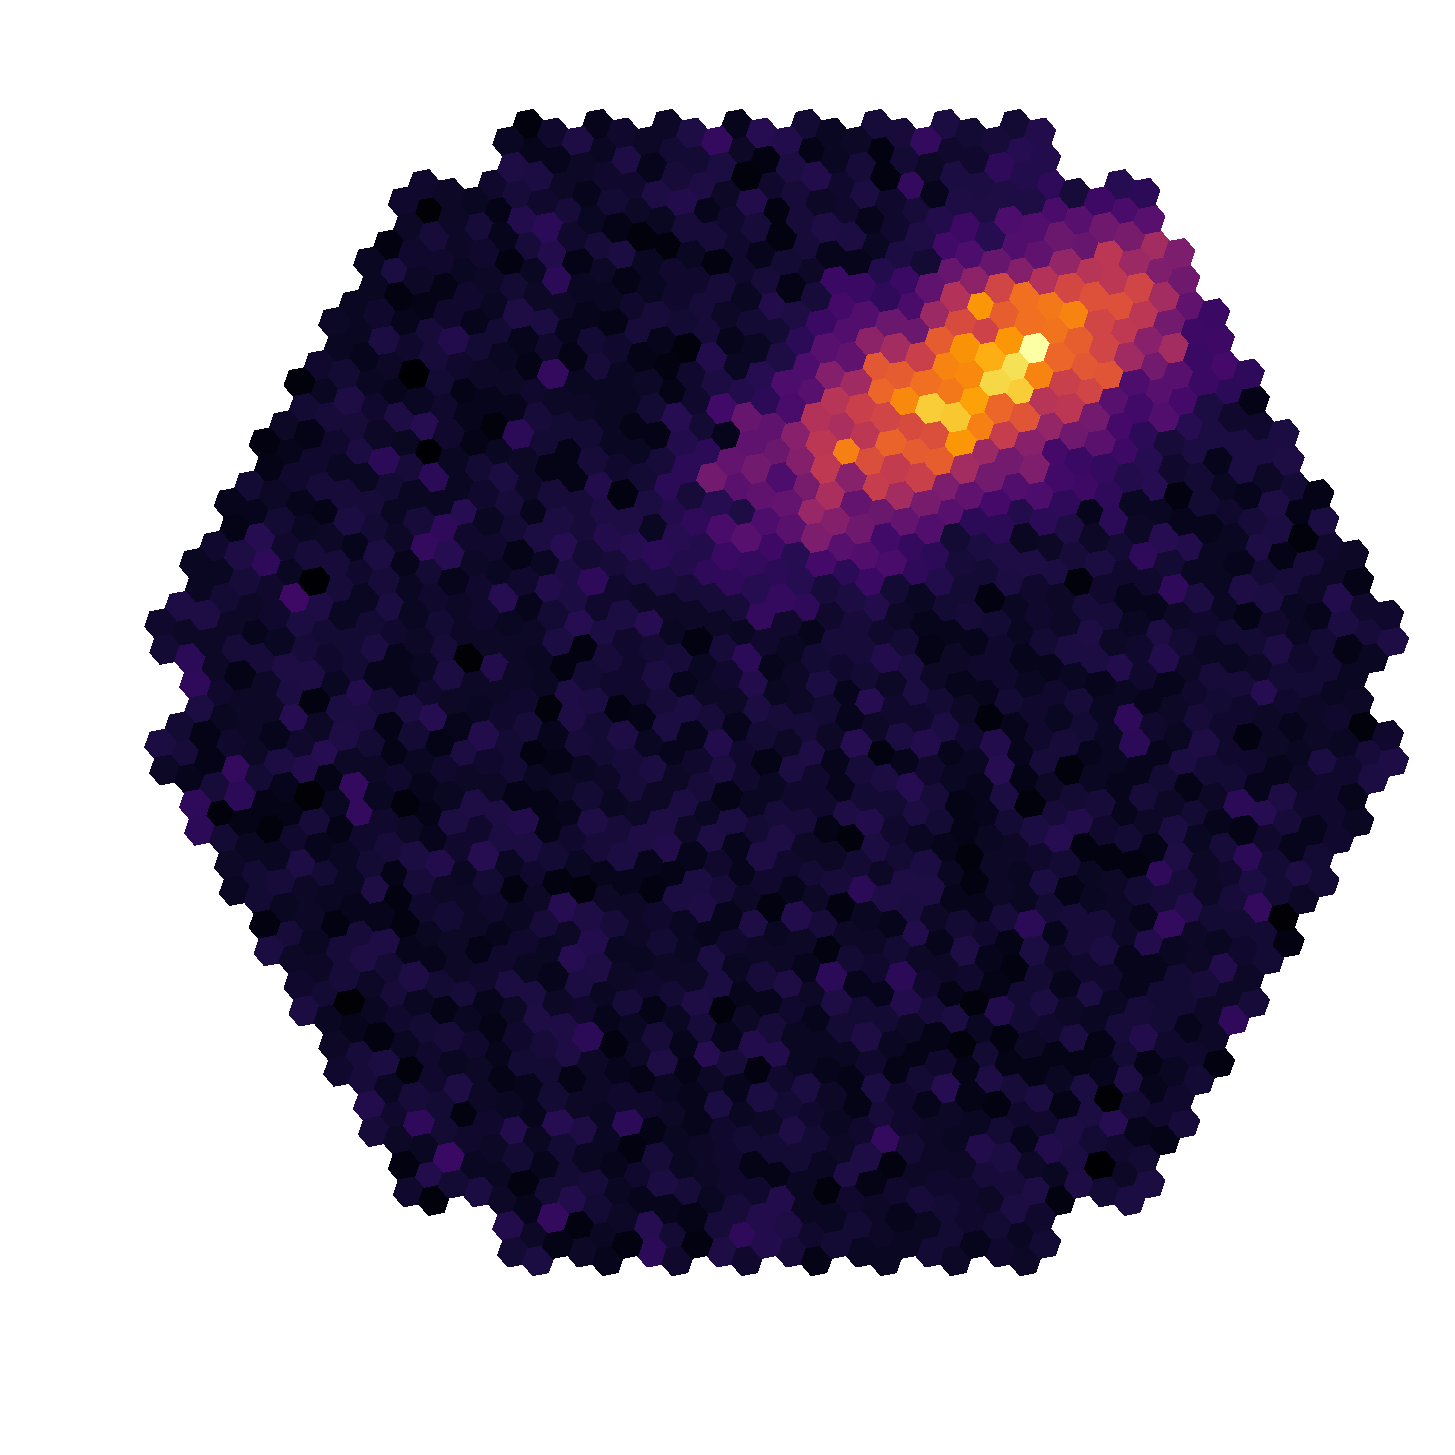
\includegraphics[width=0.9\linewidth]{../Plots/hillas_raw.pdf} 
        %\caption{Caption1}
        \label{fig:3}
    \end{subfigure}
    \begin{subfigure}{0.3\textwidth}
        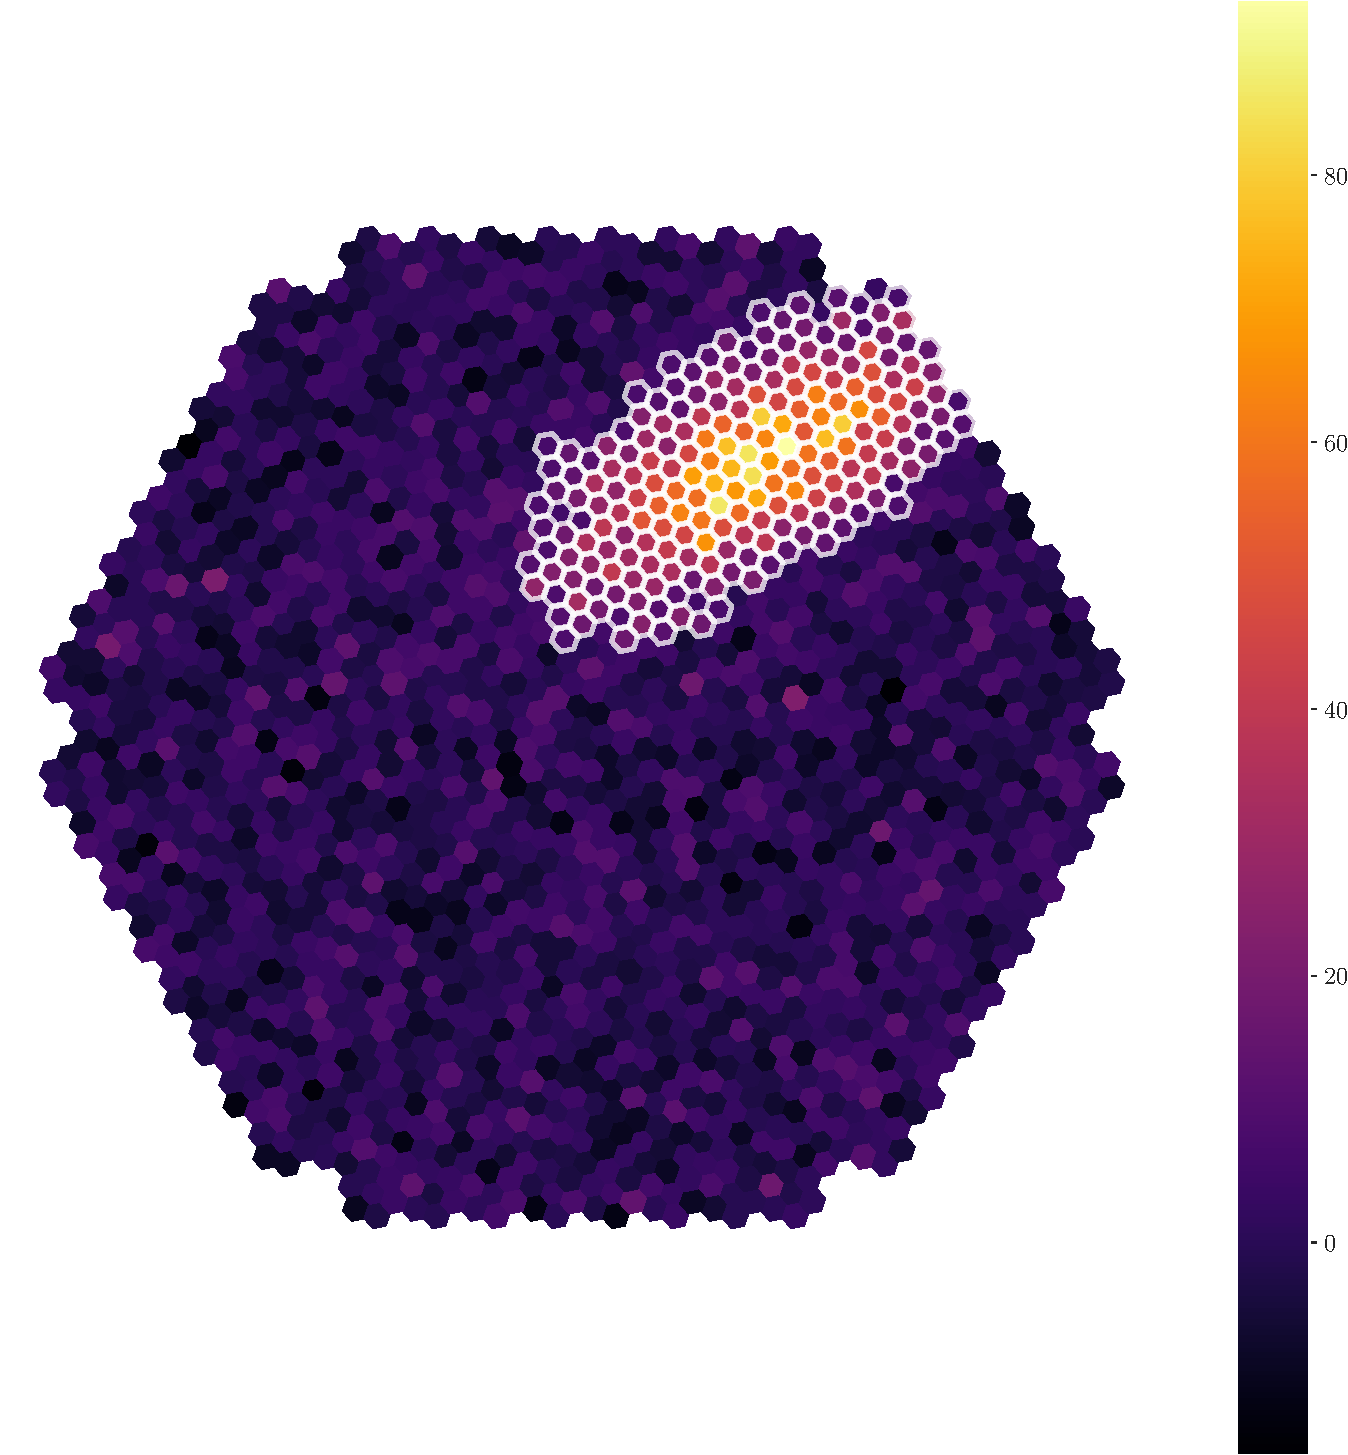
\includegraphics[width=0.9\linewidth]{../Plots/hillas_cleaned.pdf}
        %\caption{Caption 2}
        \label{fig:2}
    \end{subfigure}
    \begin{subfigure}{0.3\textwidth}
        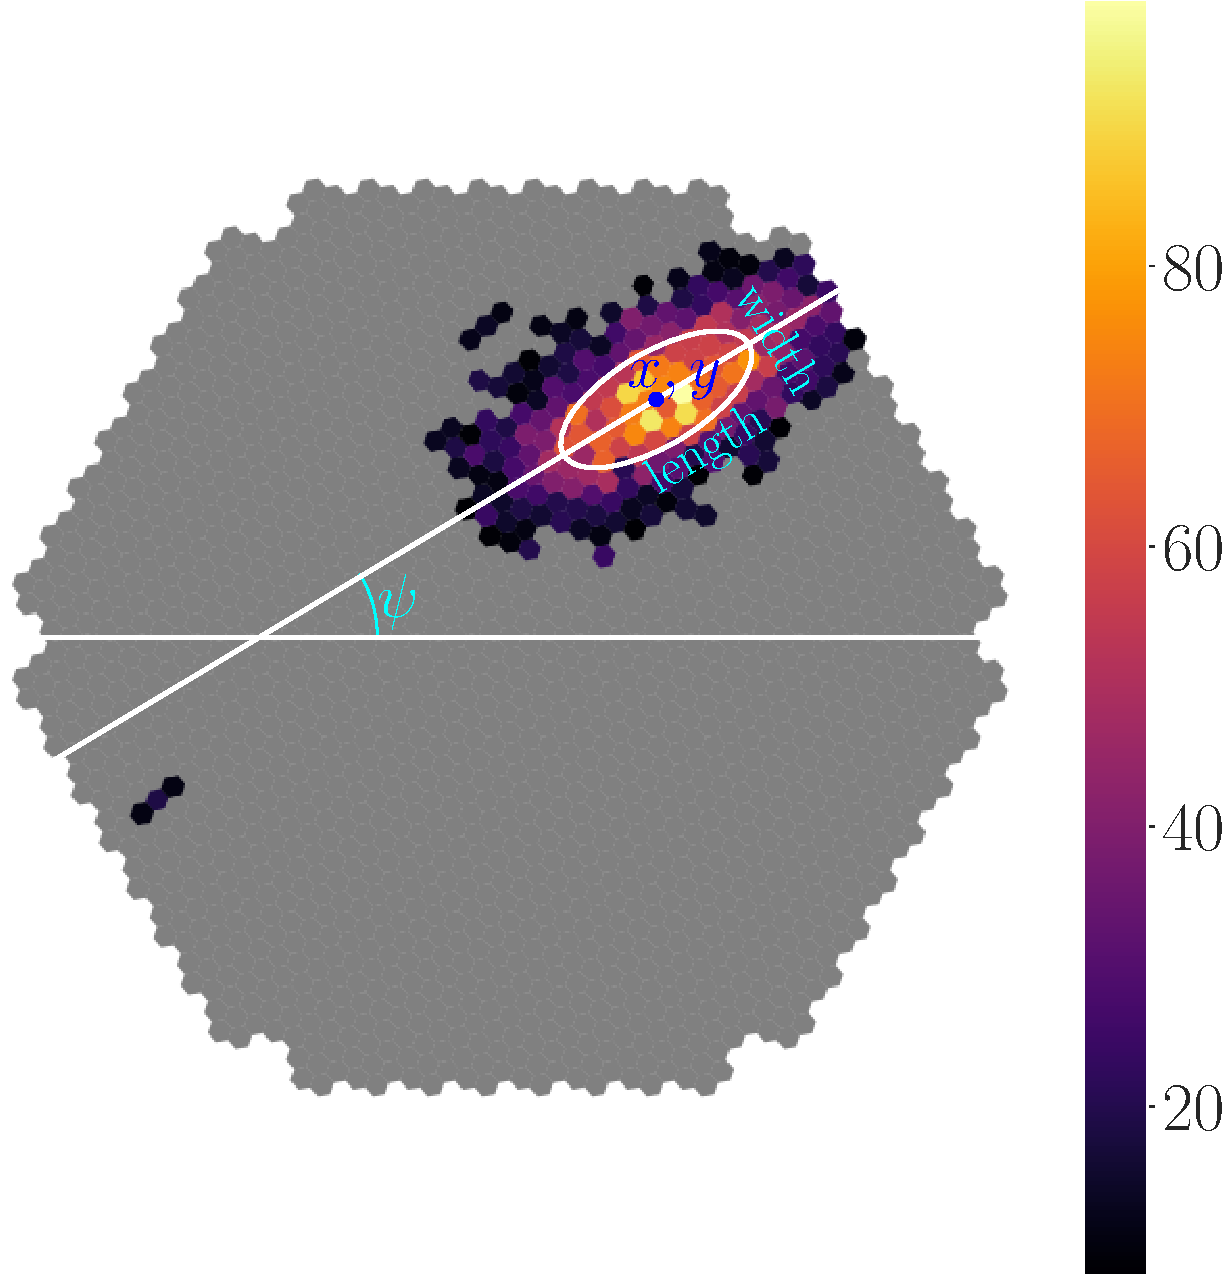
\includegraphics[width=0.9\linewidth]{../Plots/hillas_cleaned_params.pdf} 
        %\caption{Caption1}
        \label{fig:1}
    \end{subfigure}
    \caption{wrong pics}
    \label{fig:disp_magic}
\end{figure}



The analysis software ctapipe (citation) that gets developed for
CTA, currently implements a slightly different, geometric approach.
The so called HillasReconstructor constructs hillas planes
from the pointing of the telescopes and the reconstructed hillas parameters
and calculates a weighted average of the intersections.

A schematic illustration is given by figure \ref{fig:hillas_reco}

\begin{figure}
    \centering
    \includegraphics[width=0.8\textwidth]{./Plots/Histogramm.pdf}
    \caption{HillasReconstructor}
    \label{fig:hillas_reco}
\end{figure}

Obviously this requires at least two triggered telescopes.
On the other hand this approach scales
very well for high numbers of telescopes and
also provides an etimation of the interaction height.
Competitive performance is generally reached
at around 3 telescopes (citation).


A DISP-based method for CTA is required to perform a reconstruction on
events with an arbitrary number of triggered telescopes.
As this scaling can be somewhat nontrivial in some cases I am gonna
compare a few different approaches and compare the performances
with a single telescope DISP-prediction and the HillasReconstructor.
Calculation of the DISP and SIGN at
telescope-level is performed using the aict-tools(citation).
In the background random forest are constructed for both the
DISP-regression and the SIGN-classification.
For combining the individual predictions to an array level prediction
the following methods will be compared:

\textbf{mean}
The correct estimation is deciced at telescope-level usign the
SIGN-information. The mean of all positions gets calculated as
array prediction.
This implicitly assumes all SIGN's are correctly classified as
wrong classification leads to very far off predictions.
As this is not the case and accuracies >80\% are not realistic,
this naive approach is expected to perform not better than the individual
telescope predictions.
It is mainly included as a benchmark to emphasize the problems
that follow the reconstruction ambiguity and are not present for
energy regression or g/h separartion.


\textbf{outlier resistant average estimation}
%\textbf{median}
Assuming that most events get classified correctly, a calculation of
the average of all telescope-predictions might still be successful if
events with wrong reconstructed SIGN's are not taken into account.
The simplest way to perform an outlier resistant reconstruction
would be to take the median instead of the mean.
Another possible algorithmus iteratively calculates
the median and and standard deviation of the cluster and removes
outliers based on their distance to the median.
This algorithmus is implemented as "sigma_clipped_stats" in astropy (citation).

\textbf{Pairwise combination (MAGIC-based)}
Since algorithms for choosing the correct points exist for the
case of two telescopes, one could treat each pair of observations 
the same way the magic telescopes do to resolve the head-tail-ambiguity.
The results of all of these pairs could then be combined by taking the mean 
or median.
The following figure \ref{fig:disp_cta_magic} illustrates the general idea of iteratively 
choosing two of the triggered telescopes.

\begin{figure}
    \begin{subfigure}{0.3\textwidth}
        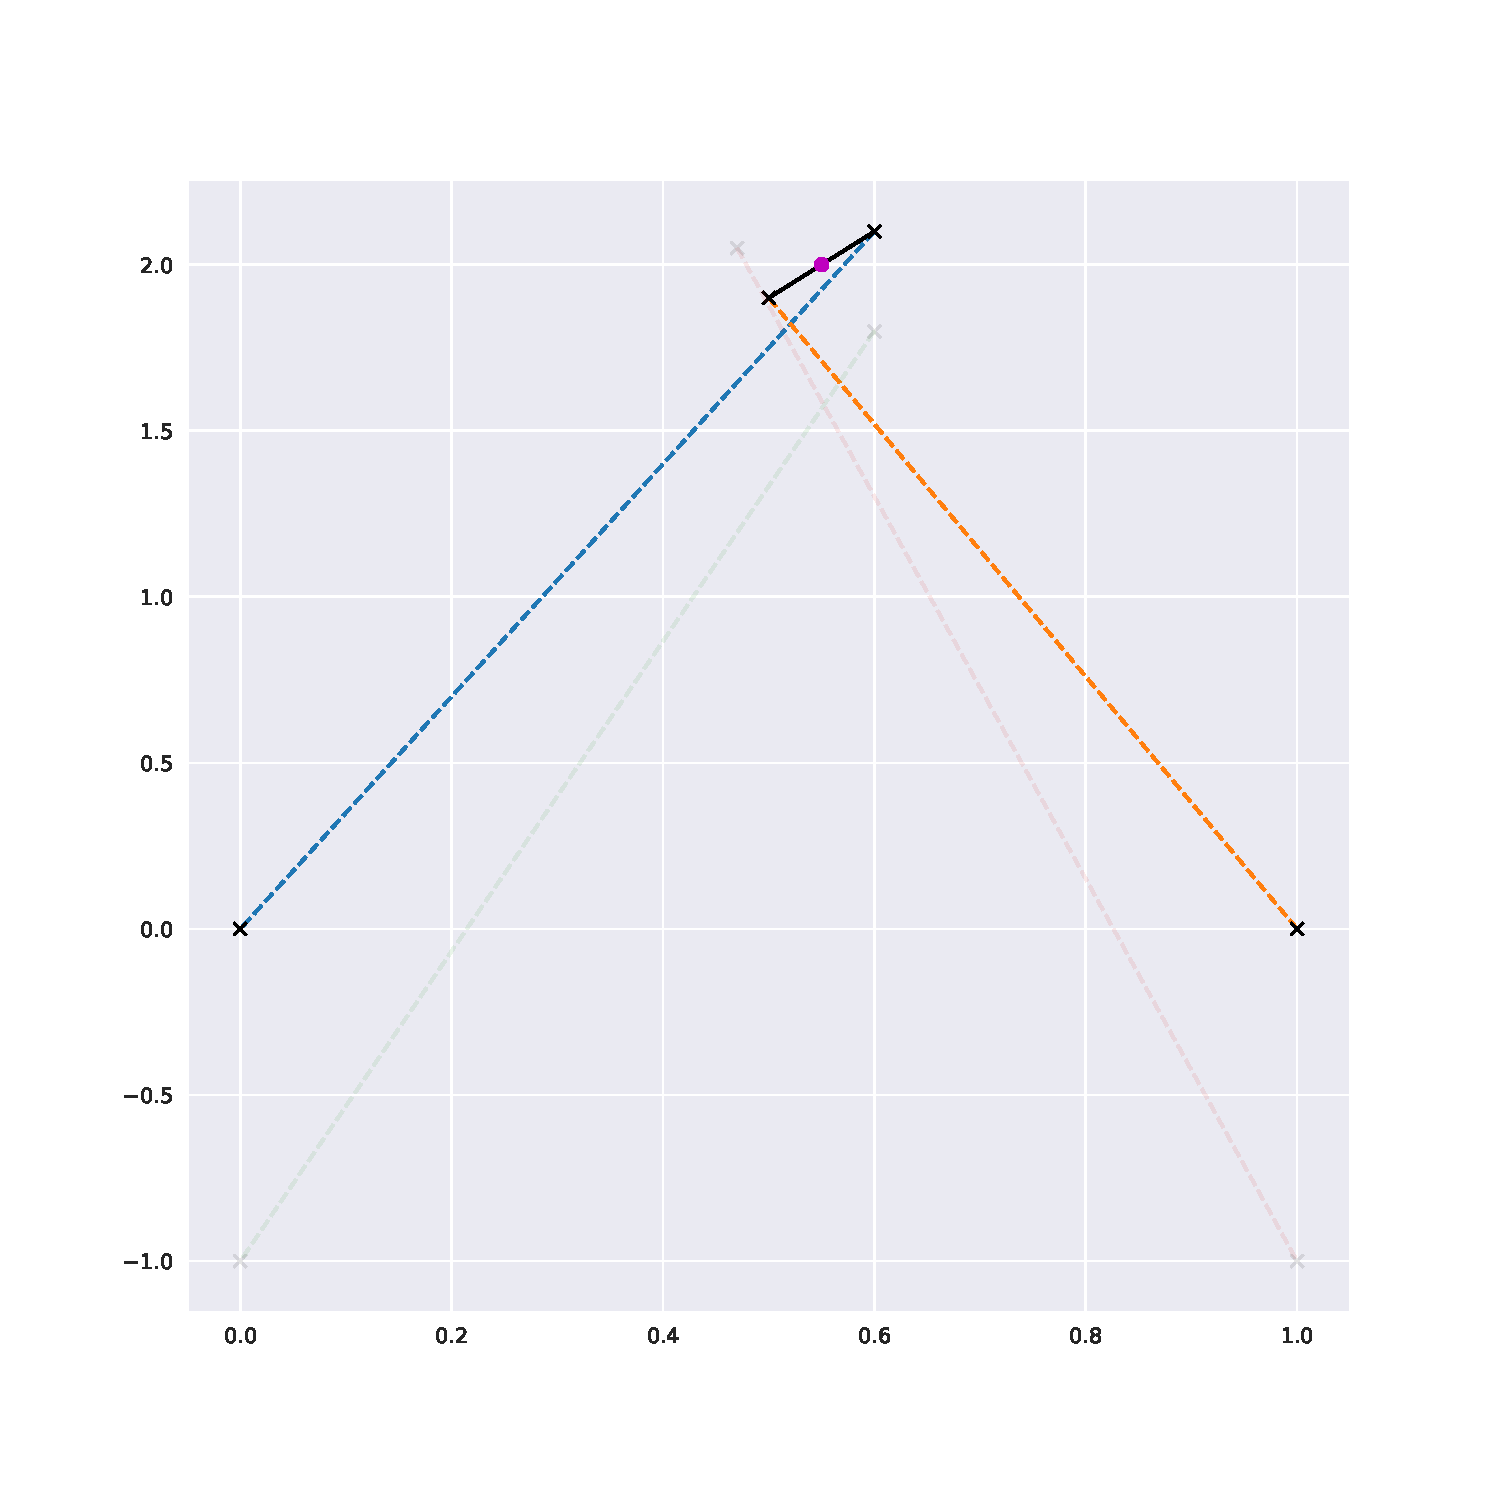
\includegraphics[width=0.9\linewidth]{../Plots/stereo_magic_1.pdf} 
    \end{subfigure}
    \begin{subfigure}{0.3\textwidth}
        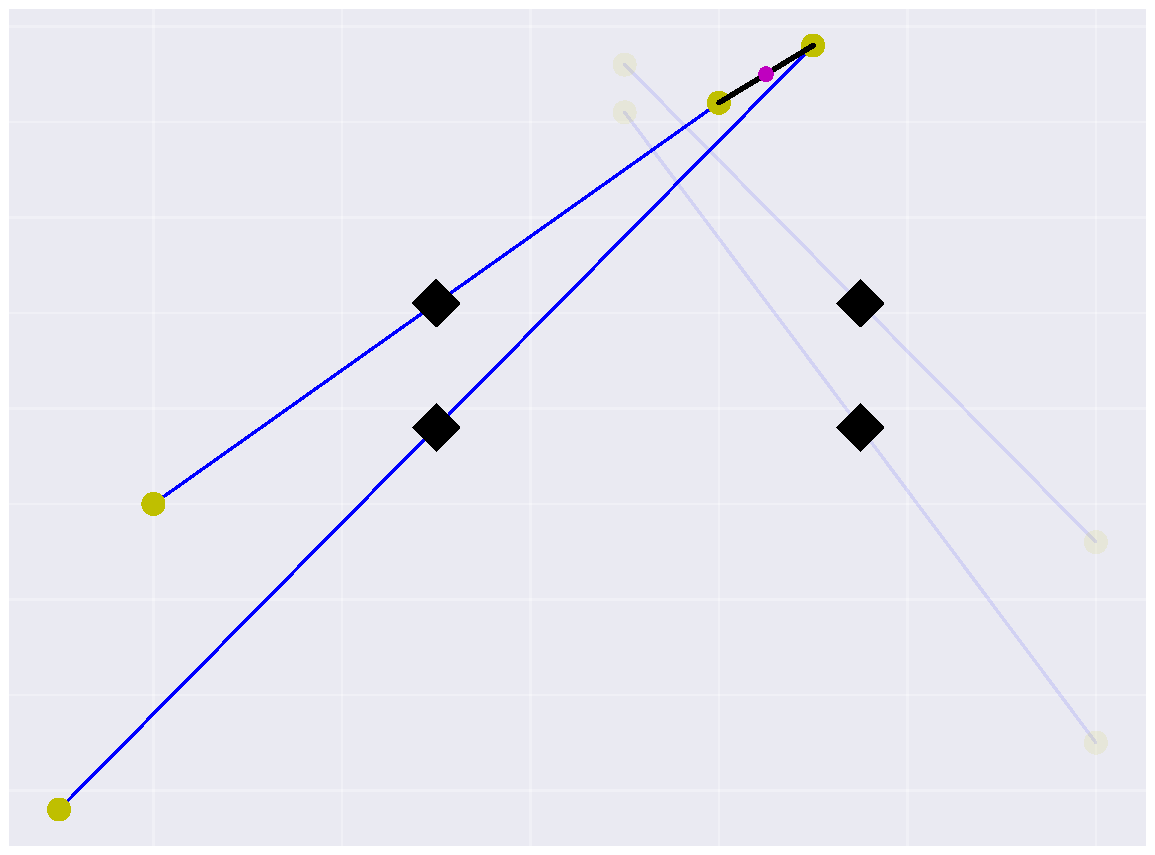
\includegraphics[width=0.9\linewidth]{../Plots/stereo_magic_2.pdf}
    \end{subfigure}
    \begin{subfigure}{0.3\textwidth}
        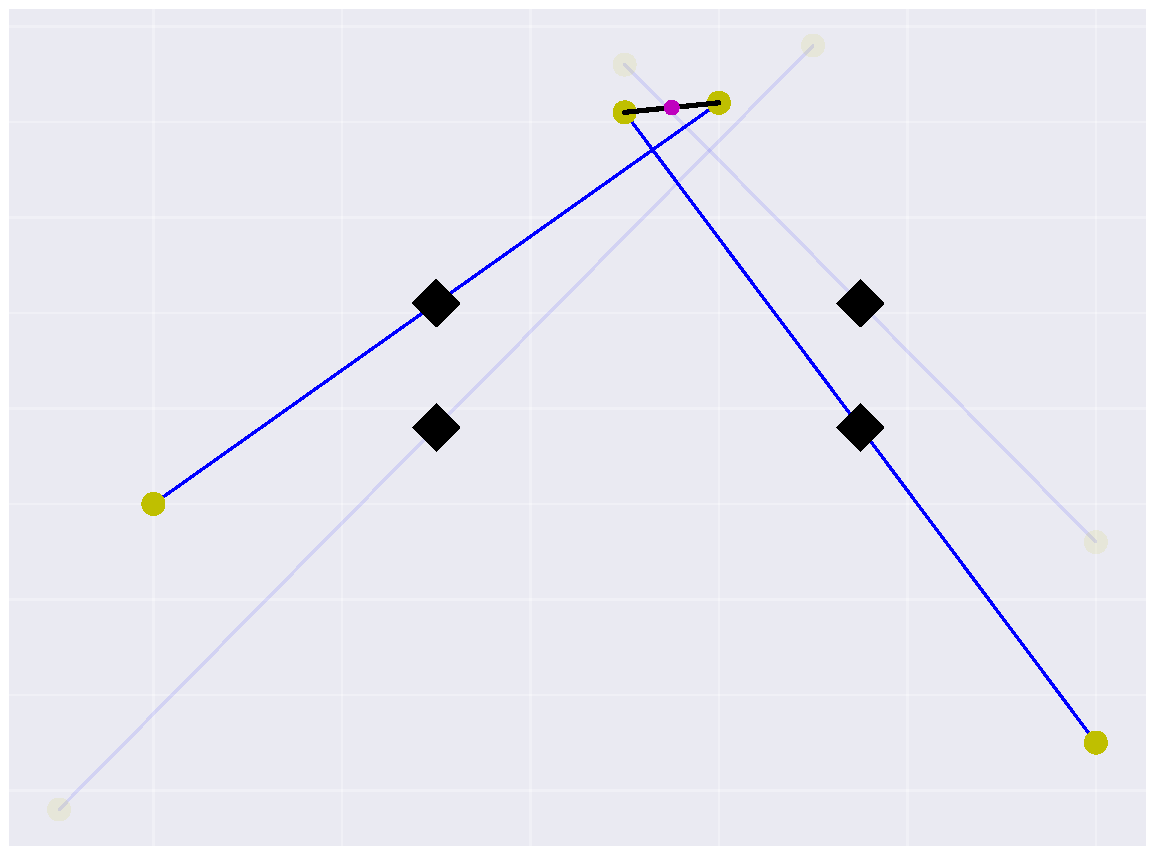
\includegraphics[width=0.9\linewidth]{../Plots/stereo_magic_3.pdf} 
    \end{subfigure}
    \begin{subfigure}{0.3\textwidth}
        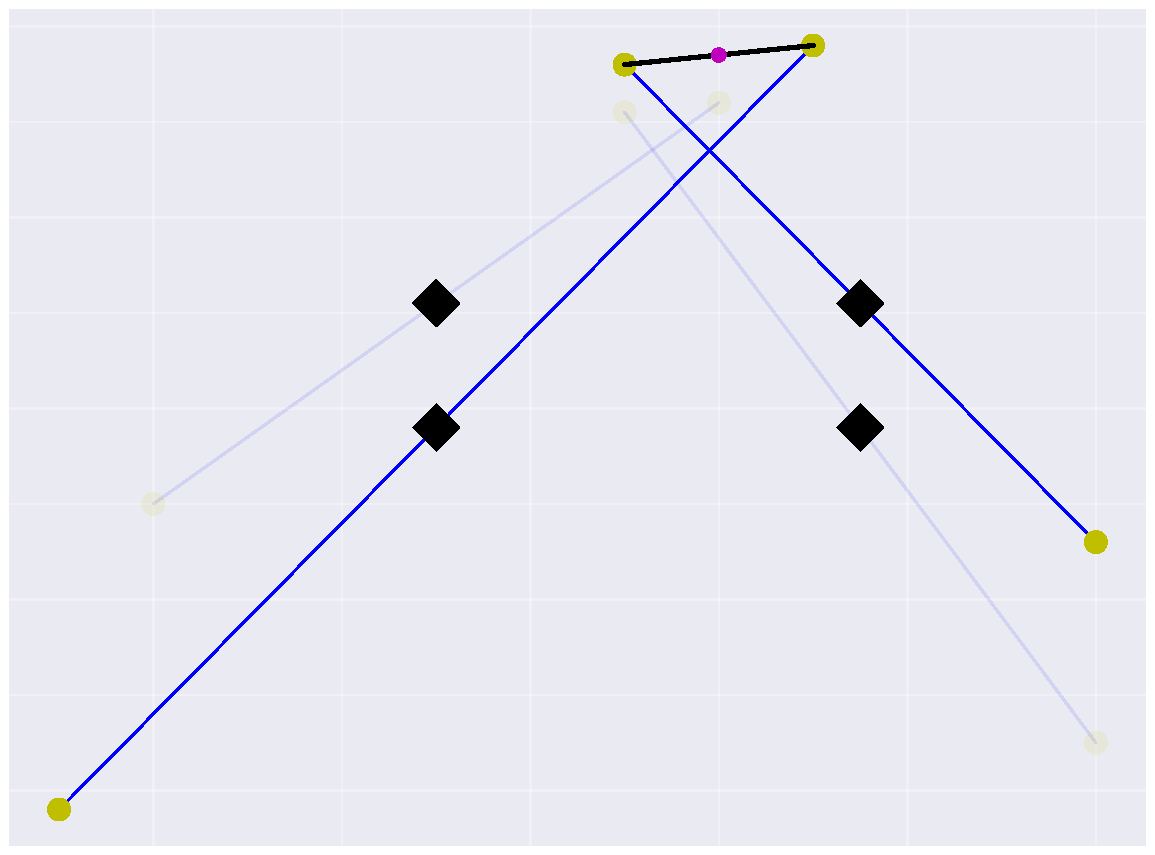
\includegraphics[width=0.9\linewidth]{../Plots/stereo_magic_4.pdf} 
    \end{subfigure}
    \begin{subfigure}{0.3\textwidth}
        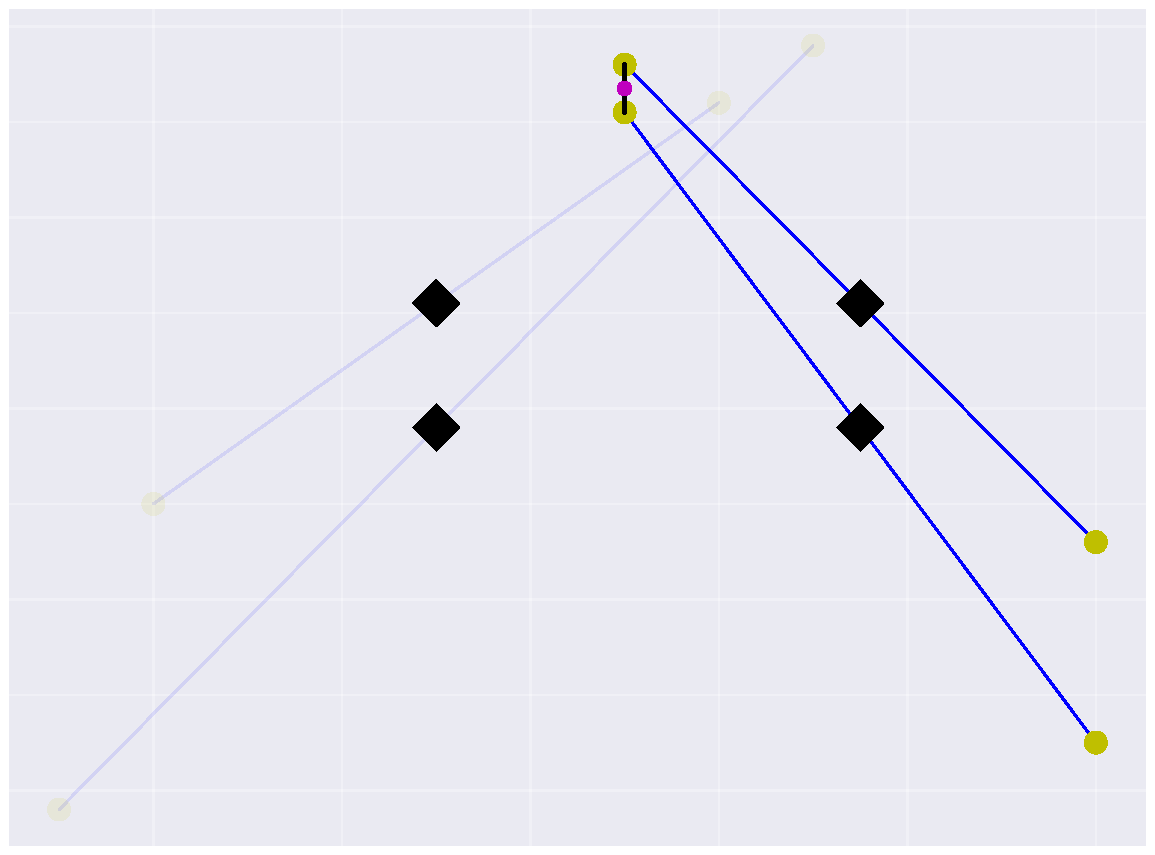
\includegraphics[width=0.9\linewidth]{../Plots/stereo_magic_5.pdf}
    \end{subfigure}
    \begin{subfigure}{0.3\textwidth}
        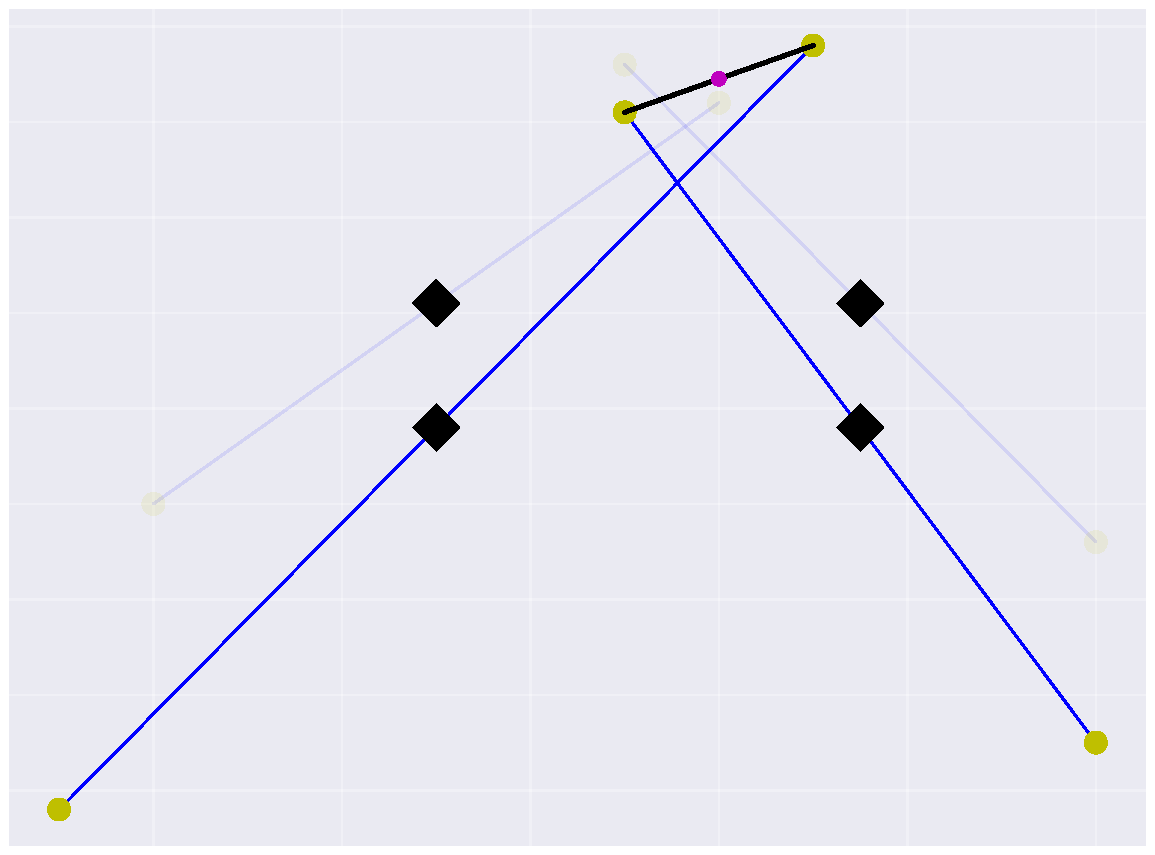
\includegraphics[width=0.9\linewidth]{../Plots/stereo_magic_6.pdf} 
    \end{subfigure}
    \caption{Its a king of magic}
    \label{fig:disp_cta_magic}
\end{figure}

- idea
- hope


\textbf{HESS-method}
Das ist mega nice, aber braucht error estimates.

\textbf{Veritas-method}
Since the predictiosn with the correct sign should cluster around the true source
position and the misclassified predictions should be less densely clustered, we 
can formulate our problem as: Find the biggest cluster of points and average these.
This sounds like a textbook application of clustering algorithms.
The algorithm of choice for this work has been the DBSCAN algorithm (citation)
as implemented in sklearn (citation). The algorithm requires a minimal distance to 
be defined for points to count as neighbours. It then collects clusters and 
treats non associated points as background. We then take the cluster with the most 
points in it and average over these points.

The choice of a minimal distance directly influences the performance 
of the algorithm as too small of a distance leads to points left out and potentially 
wrong identification of the main cluster as clusters get small while 
choosing the mininmal distance too big includes misclassified predictions 
making the averaging harder.

\begin{figure}
    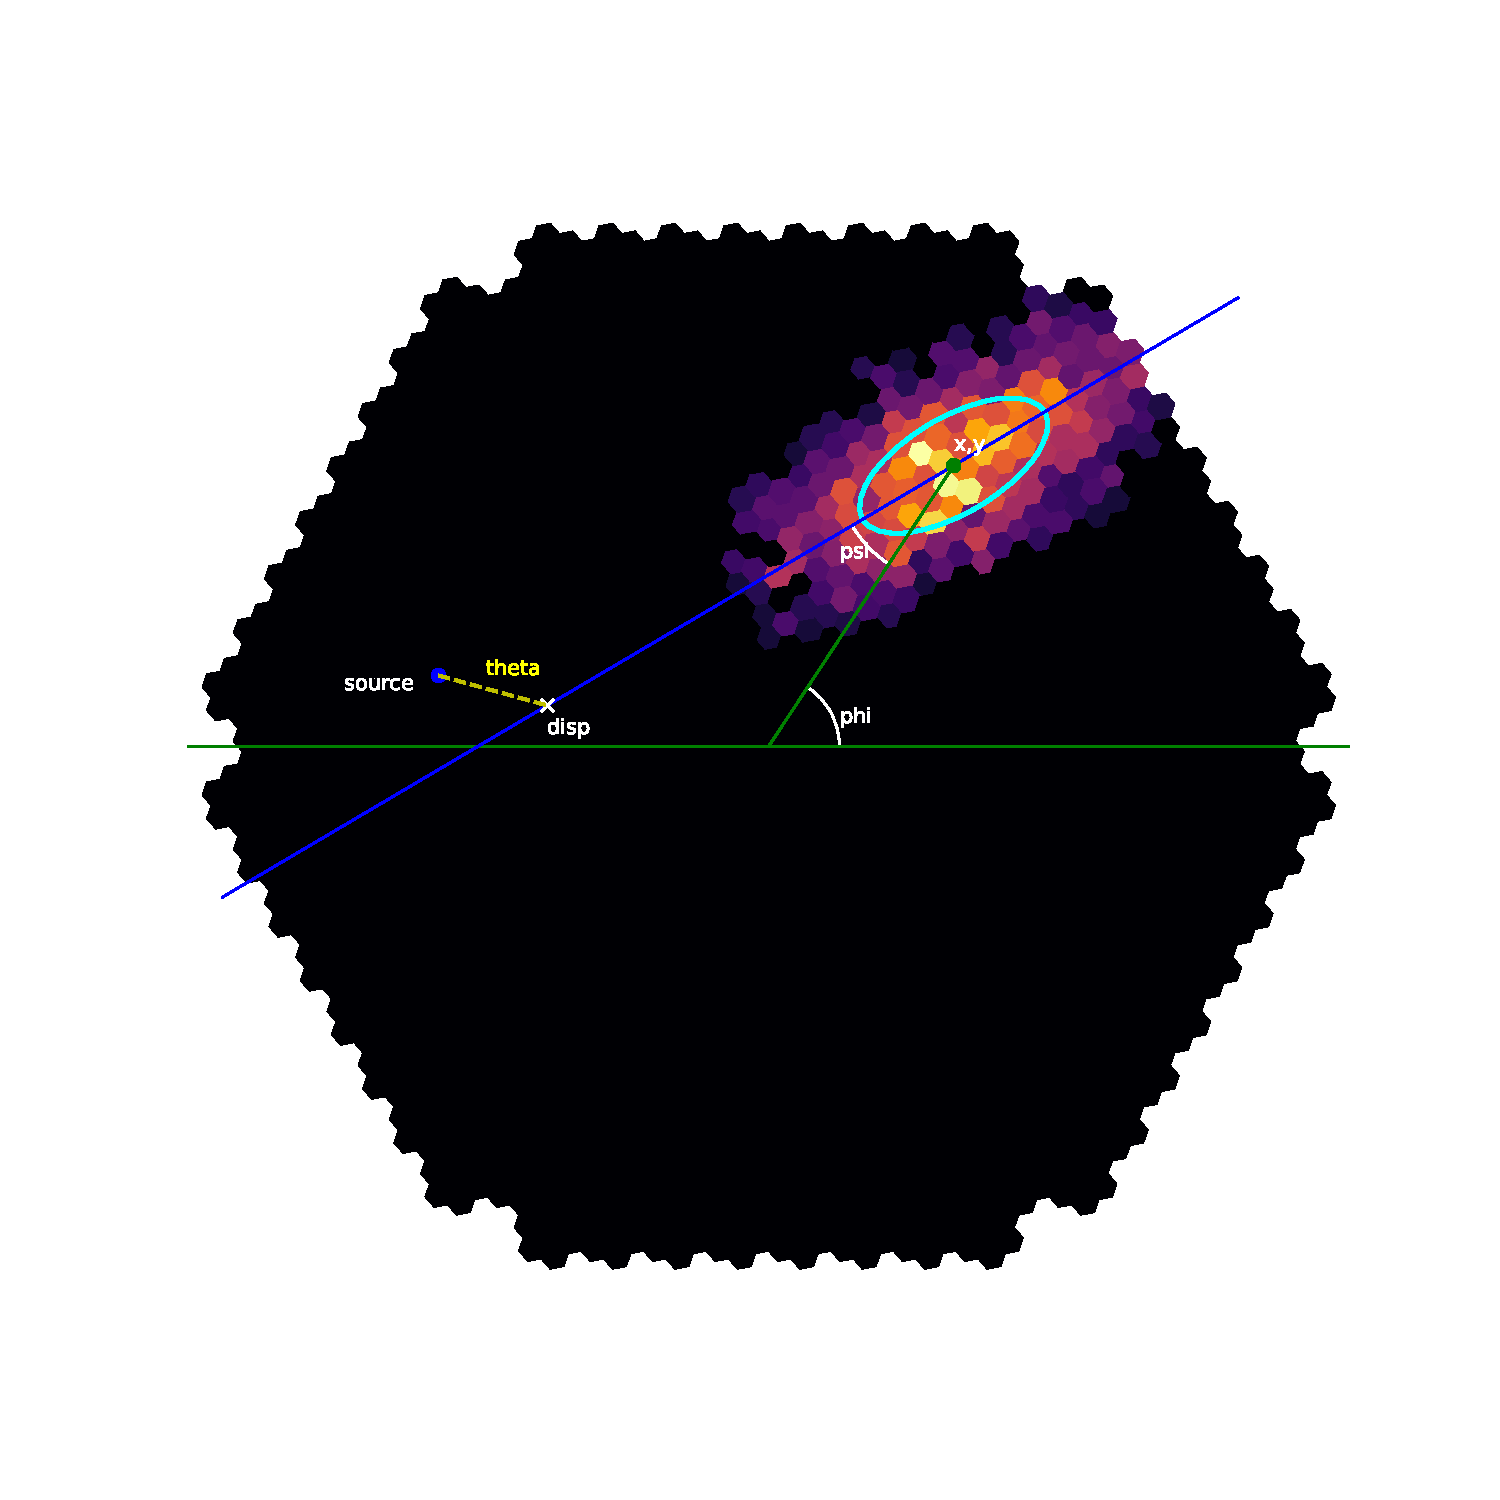
\includegraphics[width=0.9\linewidth]{../Plots/hillas_complete.pdf}
    \caption{Wrong pic!}
    \label{fig:disp_amb}
\end{figure}


\begin{figure}
    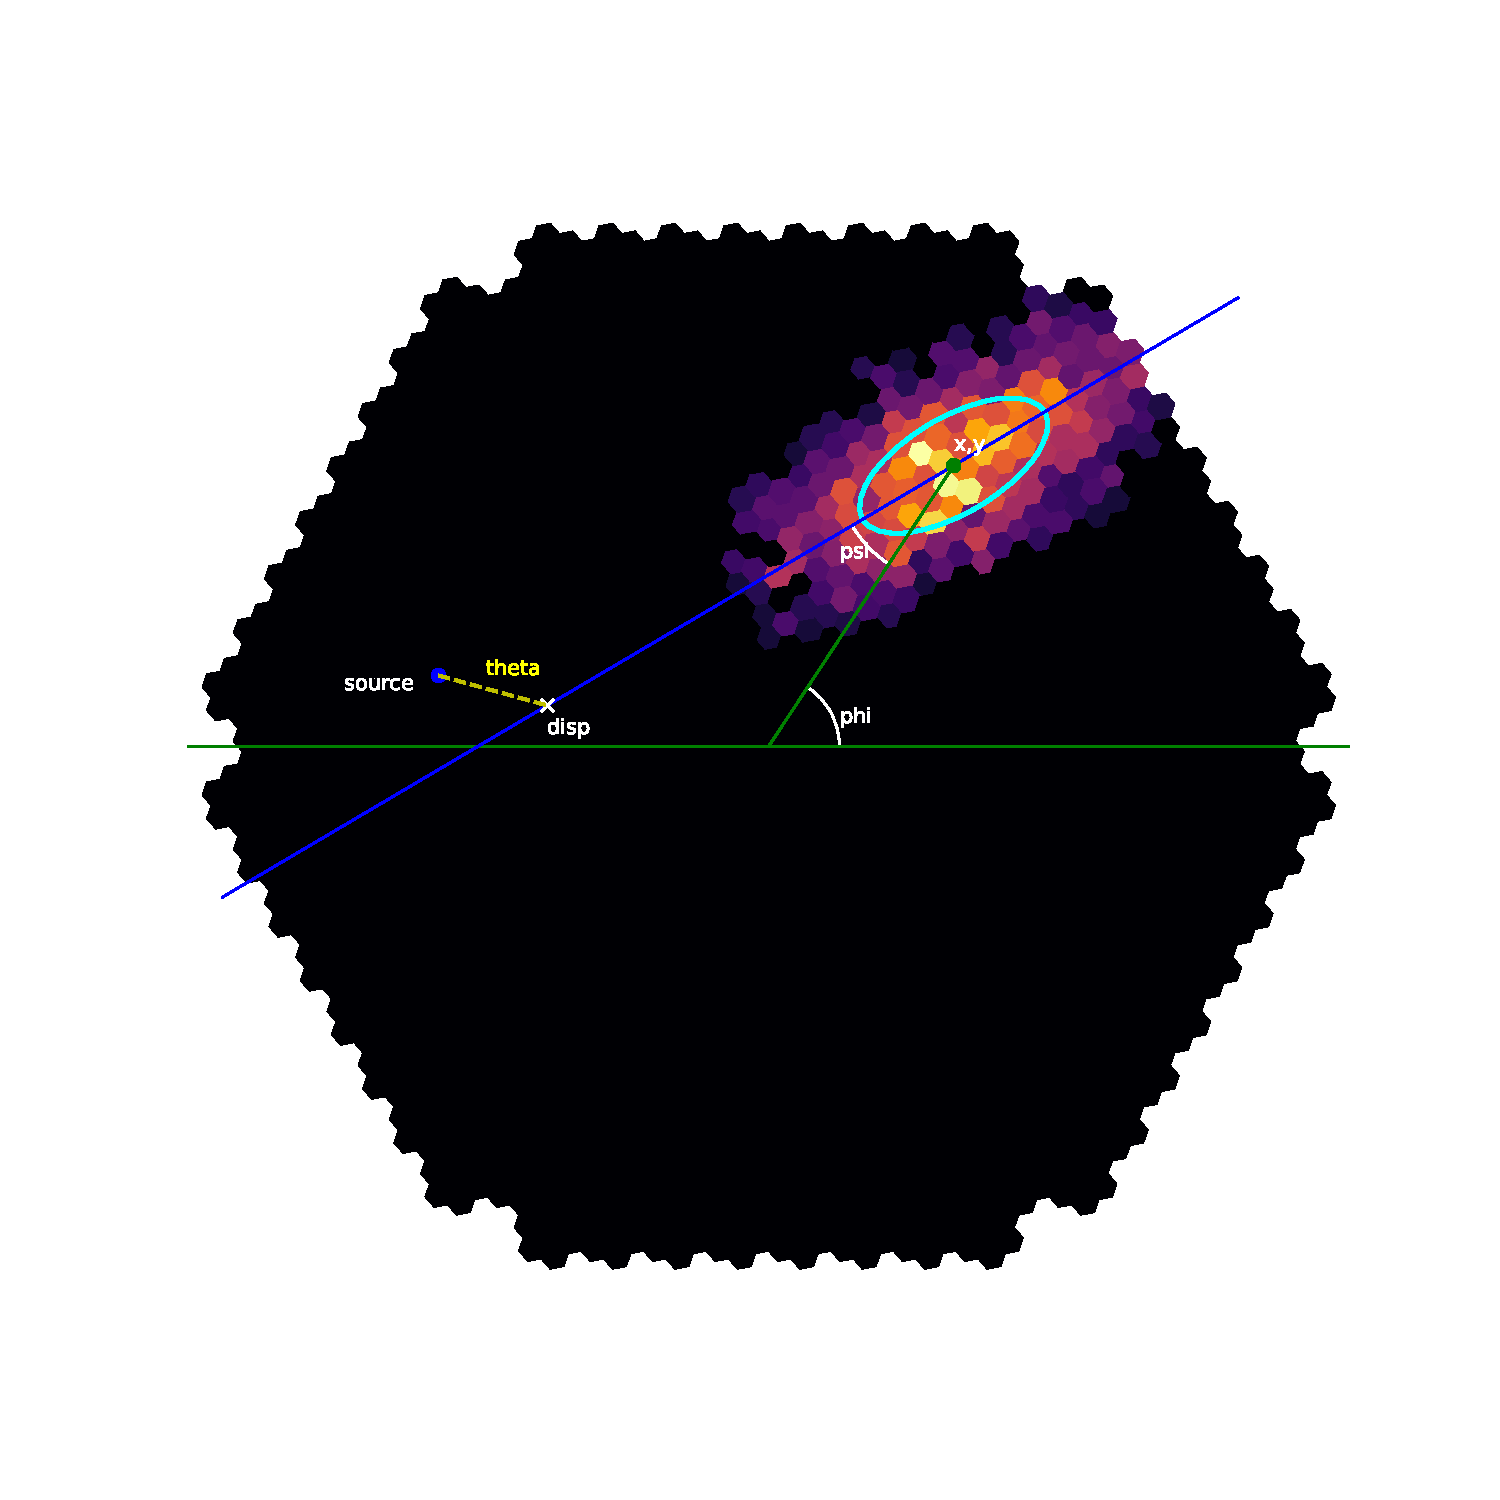
\includegraphics[width=0.9\linewidth]{../Plots/hillas_complete.pdf}
    \caption{Wrong pic!}
    \label{fig:disp_amb}
\end{figure}


\section{Analysed Data}
\subsection{Corsika Simulation}
\subsection{Training, Testing, mismatches und so, weniger telescope daten bei weniger teleskopen! duh... aber wichtig für statistik.}
